\section{Image symmetry implementation}
\newcommand\cbw{\mathit{CBW}}
\newcommand\gbw{\mathit{GBW}}

\subsection{Invariant Layers}
\subsubsection{CBW Layer}
As described in section \ref{sec:theoretical_equiinv}, in order to construct a network
invariant to some group of transformations, either the first layer has to be
invariant or first layers have to be equivariant with an invariant layer
following them. In this section we construct networks of both of these types.
First we need to construct layers invariant to changes in
contrast, brightness, color balance and gamma correction as defined in
\ref{sec:transformations}. If possible it would be best to use a single function
invariant to all of these transformations at once. While we weren't able to come
up with such layer, we can do the next best thing and build layers invariant to
three of these transformations.
We show that standard instance normalization is invariant to contrast, brightness
and color balance changes.

Instance normalization layer $\mathit{CBW}$ transforms each channel
$X_c$ of image $X$ by:
$$ \mathit{CBW}(X_c) = \frac{X_c-E[X_c]}{\sigma(X_c)} $$
where $E[X_c]$ is mean value of $X_c$ and $\sigma$ is its standard deviation.
Each instance in batch is normalized separately.
\textit{CBW} is invariant to changes in contrast $\mcc$:
\begin{align*}
    \mathit{CBW}(\mcc_a(X)_c) &=
    \frac{aX_c+(1-a)E[X]_c - E\left[aX_c+(1-a)E[X]_c\right]}{\sigma(aX_c+(1-a)E[X]_c)} \\
    &= \frac{aX_c+(1-a)E[X]_c - aE[X_c]-(1-a)E[X]_c}{a\sigma(X_c)} \\
    &= \frac{aX_c-aE[X_c]}{a\sigma(X_c)} \\
    &= \frac{X_c-E[X_c]}{\sigma(X_c)} \\
    &= \mathit{CBW}(X_c)
\end{align*}
Similarly for brightness changes $\mathcal{B}$:
\begin{align*}
    \mathit{CBW}(\mathcal{B}_a(X)_c) &=
    \frac{aX_c - E\left[aX\right]_c}{\sigma(aX_c)} \\
    &= \frac{aX-aE[X_c]}{a\sigma(X_c)} \\
    &= \frac{X_c-E[X_c]}{\sigma(X_c)} \\
    &= \mathit{CBW}(X_c)
\end{align*}
Color balance changes $\mathcal{W}$ act on individual channels in the same way
$\mathcal{B}$ does so:
\begin{align*}
    \mathit{CBW}(\mathcal{W}_T(X)_c) &=
    \frac{T_cX_c - E\left[T_cX_c\right]}{\sigma(T_cX_c)} = \\
    &= \frac{T_cX-T_cE[X_c]}{T_c\sigma(X_c)} = \\
    &= \frac{X_c-E[X_c]}{\sigma(X_c)} = \\
    &= \mathit{CBW}(X_c)
\end{align*}
Therefore any neural network with $\mathit{CBW}$ as first layer
makes the network invariant to considered image transformations.
We denote this type of networks as \{model-name\}+InCBW0, e.g. Plain+InCBW0 or
RotEq+InCBW0. Where 0 refers to placement of the invariant layer at the
beginning of the network. We also consider invariant networks with $\mathit{CBW}$
layer placed further down the processing stream. As mentioned earlier,
constructing such network requires all layers before $\mathit{CBW}$ to be
equivariant. Since the equivariance to changes in color balance is not defined,
we focus on contrast and brightness. In the next section \ref{sec:equ_models} we
present variants of common layers like convolution or pooling equivariant to
these transformations. We use these components to construct invariant networks
denoted InB1, InB2, InB3. Numbers again refer to
placement of the $\mathit{CBW}$ layer -- the higher the number, the deeper
invariant layer is placed.

\subsubsection{GBW Layer}
Just like $\cbw$ layer is invariant to changes in contrast,
we can construct similar normalization layer $\gbw$ invariant to changes in
gamma:
\begin{equation}
    \gbw(X_c) = \frac{\log{X_c}-E[\log{X_c}]}{\sigma(\log{X_c})}
    \label{eq:GBW}
\end{equation}
where $\log(X)$ is entrywise logarithm of $X$. The base of the
logarithm is not very important -- invariant behaviour doesn't depend on its
value; in implementation we use base $e$.
Now let us assume that we're given an image -- $3\times H \times W$ tensor --
with strictly positive values..
Operators $\mathcal{G}$, $\mathcal{B}$ and $\mathcal{W}$ act on it entrywise, so
we can as well analyze transformation of individual channels of the image.
Let $X$ be a single channel.
We prove \ref{eq:GBW} is invariant to gamma, brightness and color balance
changes. $\mathcal{B}$ and $\mathcal{W}$ transform single channel in the same
way, by multiplication,
so we only need proofs for $\mathcal{G}$ and $\mathcal{B}$:

\begin{align*}
    \gbw(\mathcal{G}_a(X)) &=
    \gbw(X^a) \\
    &= \frac{\log(X^a)-E[\log(X^a)]}{\sigma(\log(X^a))} \\
    &= \frac{a\log(X)-E[a\log(X)]}{\sigma(a\log(X))} \\
    &= \frac{a\log(X)-aE[\log(X)]}{a\sigma(\log(X))} \\
    &= \frac{\log(X)-E[\log(X)]}{\sigma(\log(X))} \\
    &= \gbw(X)
\end{align*}

\begin{align*}
    \gbw(\mathcal{B}_a(X)) &=
    \gbw(aX) \\
    &= \frac{\log(aX)-E[\log(aX)]}{\sigma(\log(aX))} \\
    &= \frac{\log(X)+\log(a)-E[\log(X)+\log(a)]}{\sigma(\log(X)+\log(a))} \\
    &= \frac{\log(X)+\log(a)-E[\log(X)]-\log(a)}{\sigma(\log(X))} \\
    &= \frac{\log(X)-E[\log(X)]}{\sigma(\log(X))} \\
    &= \gbw(X)
\end{align*}

There is however slight technical issue with definition \ref{eq:GBW}.
Since images contain values from interval $[0;1]$,
taking their logarithm directly is impossible because of
cells containing $0$. This problem is solved easily by adding some small constant value
$\epsilon$ to every cell before computing logarithm. The exact definition
is then the following:
\begin{equation}
\gbw_{\epsilon}(X_c) =
    \frac{\log(X_c+\epsilon)-E[\log(X_c+\epsilon)]}{\sigma(\log(X_c+\epsilon))}
\end{equation}
To be precise, this small correction breaks the invariance properties.
We can however treat $X_c+\epsilon$ as a new input of the network
and $\gbw_{\epsilon}$ is then invariant to this new input.
$\epsilon$ is small so $X_c$ and $X_c+\epsilon$ are very similar (or even
indistinguishable to human eye), so they should be labeled by the network as
belonging to the same class anyway. In implementation we use
$\epsilon=\frac{1}{255}$ -- the smallest possible difference between pixel
values.
\\ Due to logarithm only being defined for positive values, we place
$\mathit{GBW}$ layer only at the very beginning of networks. This type of models
is marked as \{model-name\}+InGBW0.
In order to prevent division by $0$ in case of constant channels, it's necessary
to add another small constant to denominator -- we use value $10^{-6}$. We do
the same in case of $\mathit{CBW}$ layer. These approximations also cause loss of
strict invariance, but again, values are very small so behaviour of the layer
doesn't change that much. Precise error values are discussed in section
\ref{sec:exp_eq}.



\subsection{Equivariant models}
\label{sec:equ_models}

\subsubsection{Brightness equivariance}
Recall that layer $f$ is equivariant to
change of brightness if $ f(aX) = af(X)$ for all $a>0$.
We begin with showing that common building blocks of CNNs except for
normalization fulfill this condition:
\begin{itemize}
    \item \textbf{Convolution} is linear operation so $\mathit{Conv}(aX) =
        a\mathit{Conv}(X)$
    \item \textbf{Pooling} - all commonly used pooling layers are equivariant:
        \begin{itemize}
            \item MaxPooling amounts to taking maximal value of some set and\\
                $\max\{ax_1,ax_2,\cdots,ax_n\}=a\max\{x_1,x_2,\cdots,x_n\}$
            \item AveragePooling is precisely expectation operation $E[X]$ and
                    $E[aX] = aE[X]$
            \item EuclideanNormPooling -
                $\sqrt{(ax_1)^2+\cdots+(ax_n)^2} = a\sqrt{x_1^2+\cdots+x_n^2}$
        \end{itemize}
    \item \textbf{Activation functions} -- equivariant pointwise activation
        function is characterised by equation $f(ax) = af(x)$ for all $a>0$.
        Assuming $f$ is differentiable, $af'(ax) = af'(x)$, so $f'(ax)=f'(x)$ which
        means that $f'(a)=f'(1)$ for $a>0$ and $f'(b)=f'(-1)$ for $b<0$.
        This implies $f$ has form of generalized ReLU function
        $$f(x)=\left\{
            \begin{array}{lll}
                ax & \mbox{for some } a \in \mathbb{R} & \mbox{if } x<0 \\
                bx & \mbox{for some } b \in \mathbb{R} & \mbox{if } x \geq 0
            \end{array}\right.$$
        In particular we can use usual ReLU function.
    \item \textbf{Normalization} As shown above, instance normalization is
        invariant to brightness changes. It's easy to see that it also holds
        for BatchNormalization. This stems mainly from division by
        standard deviation which is equivariant to $\mathcal{B}$. In fact
        the numerator of $\mathit{CBW}$ is also equivariant to $\mathcal{B}_a$:
        $aX_c-E[aX_c]=a(X_c-E[X_c])$, so division by any factor involving $a$
        will break equivariance. For the same reason, we can't pass the
        numerator through any nonlinear function, e.g. square root.
        Therefore if we want the normalization to zero
        out mean value of input, we must divide by a constant, e.g. $1$.
        In implementation we use mean normalization layer
        \begin{equation}
            \mathit{MN}(X) = X - E[X]
            \label{eq:mn}
        \end{equation}
        Lack of division by standard deviation or some other dispersion metric
        might have an
        adverse effect on training procedure as there is no mechanism to keep
        values flowing through the network bounded, which might easily result in
        gradient explosion. In experiments in section \ref{sec:img_cl} we find
        the training on one of datasets indeed deteriorates, but numerical errors
        don't occur.
\end{itemize}
And so using common components with standard normalization scheme replaced by
mean normalization we can build model equivariant to brightness changes
$\mathcal{B}$. In
experiments refer to this type of architecture as BrightnessEq.

\subsubsection{Lie GCNN equivariant models}
For geometric transformations, we implement Lie GCNN
based on B-splines \cite{bekkers2019} in PyTorch framework.
The only tough part is really
implementing general operations of lifting and group convolution.
After that implementing model equivariant to any group only requires implementing operations
of these group -- taking inverse, multiplication, distance, etc.
In this way we construct models equivariant to well researched groups like
rotation and
scaling groups as well as shear transform which hasn't come up in literature
review.
\\

We now consider remaining lightning symmetries $\mathcal{C}$ and $\mathcal{G}$.
Es expected, they are not
as well-behaved as $\mathcal{B}$. While MaxPooling is also equivariant to them,
the rest
of described above layers isn't (see experiments in section \ref{sec:exp_eq}).
For the rest of this section we construct suitable
convolutional layers similar to those of Lie
GCNNs (section \ref{sec:lie_gcnn}),
activation functions and
normalization layers
equivariant to $\mathcal{C}$ and $\mathcal{G}$ operators.

\begin{itemize}
\item
The crucial part of pipeline is convolution layer. Nature of geometric
and lightning symmetries is fundamentally mathematically different. While
the first
transform coordinates or grid of image, the latter group acts pointwise on
values present in the tensor without changing coordinates in any way.
This property renders the implementation used for geometric models unfit.
Where in case of geometric symmetries different transformed locations
on original grid are sampled, in case of lightning symmetries these would be the
exact same locations. This in turn would cause creation of identical kernels and
unnecessary repetition of computation. Therefore it's obligatory to transform the
kernels in some other way consistent with equations of lifting and convolution.
We implement such mechanism using the transformations from transformation group.
That is if we want the layer to be equivariant with respect to
$\mathcal{G}_c$, then its kernel $K$ assumes values at gamma level $c$ equal to
base kernel gamma-corrected by factor of $c$:
\begin{equation}
    K(g) = K(x,c) = \mathcal{G}_c(K(x,0))
\end{equation}
where $g$ is represented as a pair (spatial location, gamma level).

\item Because of aggregation of global mean of tensor in contrast equation \ref{eq:contrast},
    designing a nontrivial pointwise activation function equivariant to
    $\mathcal{C}$ operator
    might be impossible -- value in any given cell would automatically depend on
    values of all other cells. Instead we test numerically equivariance of broad
    range of popular activation functions and find that function Softsign
    defined as $\mathit{Softsign}(x) = \frac{x}{1+|x|}$ performs fairly well.

    Operator $\mathcal{G}$ proves to be more manageable and exactly equivariant
    activation function can be found, though in the end it turns out to be
    fairly obvious. If we want $f$ to be equivariant to gamma equation \ref{eq:gamma}, then in
    particular it needs to fulfill condition $$f\left(x^c\right) =
    f\left(x\right)^c$$
    for any $x>0$ and
    $c > 0$. To obtain analytic form of $f$
    let $$f(x_0)=y_0$$ for some constants $x_0 \neq 1$ and $y_0$.
    Then $$f\left(x_0^c\right) = y_0^c$$ Now we can treat $x_0^c$ as the argument and set
    $x_0^c = z$, so $$f(z) = y_0^{\log_{x_0}z} =
    y_0^\frac{\log_{y_0}z}{\log_{y_0}{x_0}} = z^{\log_{x_0}{y_0}}$$
    but $\log_{x_0}{y_0}$ is constant, so $f$ is unique power function passing
    through $\left(x_0, y_0\right)$. For negative arguments this definition can
    be extended either symmetrically ($f(x)=f(-x)$) or antisymmetrically ($f(-x)
    = -f(x)$). We choose the latter option to enable function to assume negative
    values.
    After some trial and error we arrive at the final definition $$f_a(x)
    = s(x)|x|^a$$ with $s$ representing the sign of $x$.
    In implementation, in order to make $f$ slowly increasing, we
    choose $a=0.3$. $f_{0.3}$ is shown in the figure \ref{fig:f03}.
    Unfortunately such activation function always leads to gradient explosion
    after processing from $2$ to $20$ data batches. In consequence also in this
    case we use \textit{Softsign} function.

    \begin{figure}[h]
        \centering
        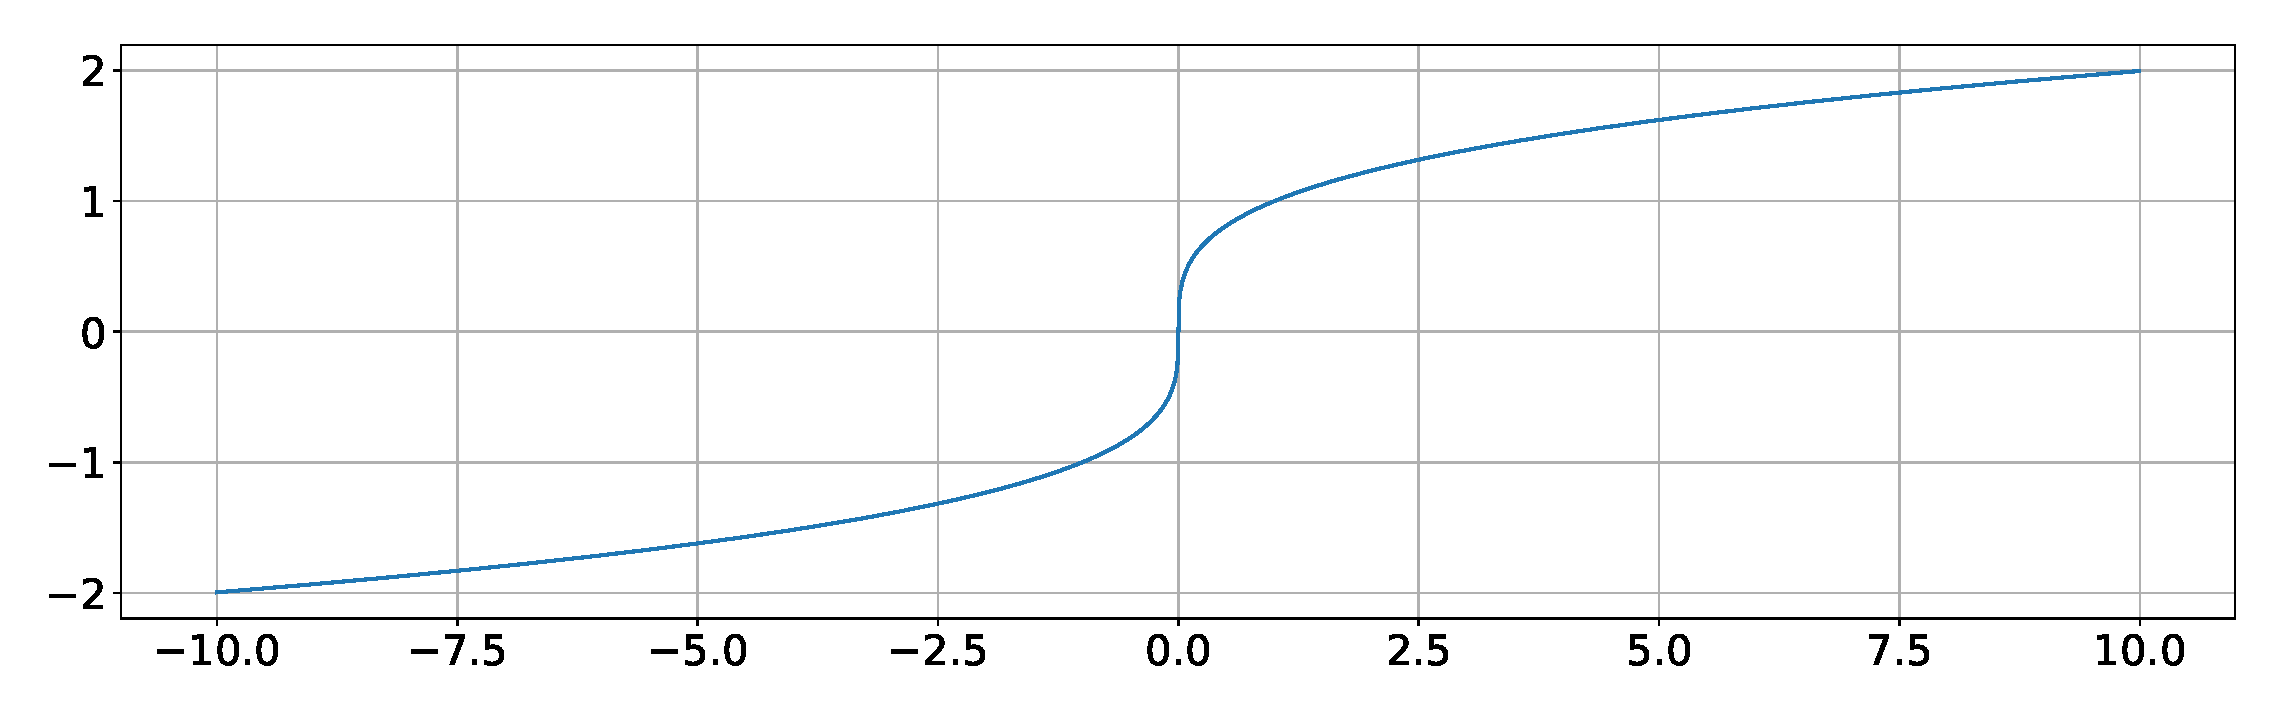
\includegraphics[width=\textwidth]{f03}
        \caption{Activation function $s(x)|x|^{0.3}$.}
        \label{fig:f03}
    \end{figure}
\item Similarly to brightness, the contrast operator $\mathcal{C}$ is
    equivariant to mean normalization and invariant to standard normalization,
    so to build an equivariant model, we need to use the mean normalization.

    Situation is a lot more complicated with gamma correction. Due to its
    highly nonlinear nature, operator
    $\mathcal{G}$ doesn't seem to be equivariant to any
    commonly used normalization layer. We test models with and without
    BatchNormalization and compare their accuracies and equivariance degrees.
\end{itemize}

